\documentclass{article}
\usepackage{pgfplots}
\pgfplotsset{compat=1.16}

\begin{document}

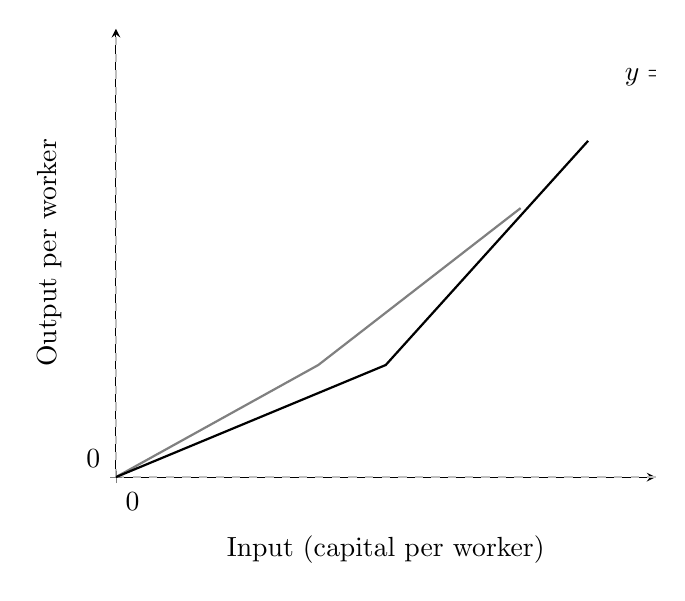
\begin{tikzpicture}
    \begin{axis}[
        axis lines = left,
        xlabel = {Input (capital per worker)},
        ylabel = {Output per worker},
        ymin=0, ymax=2,
        xmin=0, xmax=4,
        xtick=\empty,
        ytick=\empty,
        extra x ticks={0},
        extra y ticks={0},
        extra x tick style={
            majorTickLength=0pt,
            ticklabel style={},
            grid=major,
            grid style={dashed, thick}
        },
        extra y tick style={
            majorTickLength=0pt,
            ticklabel style={},
            grid=major,
            grid style={dashed, thick}
        },
        extra x tick labels={0},
        extra y tick labels={0},
        every extra x tick/.style={
            grid=major,
            grid style={dashed, thick},
            ticklabel style={anchor=north west}
        },
        every extra y tick/.style={
            grid=major,
            grid style={dashed, thick},
            ticklabel style={anchor=south east}
        },
        enlarge x limits=false,
        enlarge y limits=false
    ]
    
    % Plot the production functions
    \addplot[thick, gray] coordinates {(0,0) (1.5, 0.5) (3, 1.2)};
    \node at (axis cs:3.7, 1.8) [right] {$y=G(N)f(k)$};
    
    \addplot[thick, black] coordinates {(0,0) (2, 0.5) (3.5, 1.5)};
    \node at (axis cs:4, 2.2) [right] {$y=G(N')f(k)$};
    
    \end{axis}
\end{tikzpicture}

\end{document}